\section{\peregrine Overview} \label{sec:overview}

%% \begin{figure}[t]
%% \centering
%% \includegraphics[width=.45\textwidth]{figures/overview}
%% \caption{{\em \peregrine Architecture: main components and data structures are
%%     shaded (and in green).}}\label{fig:arch}
%% \end{figure}

\begin{figure}[t]
\centering
\includegraphics[width=.96\columnwidth]{peregrine/figures/overview.eps}
\caption{{\em \peregrine Architecture: components and data structures are
    shaded (and in green).}}\label{fig:arch}
\end{figure}

%% \begin{figure*}[t]
%% \begin{minipage}[t]{.48\textwidth}
%% \includegraphics[width=\textwidth]{figures/overview}
%% \caption{{\em \peregrine Architecture: components and data structures are
%%     shaded (and in green).}}\label{fig:arch}
%% \end{minipage}
%% \hfill
%% \begin{minipage}[t]{.50\textwidth}
%% \includegraphics[width=\textwidth]{figures/analyzer}
%% \caption{{\em Analyses performed by the analyzer.}}\label{fig:analyzer}
%% \end{minipage}
%% \end{figure*}

Figure~\ref{fig:arch} shows the architecture of \peregrine.  It has four main
components: the instrumentor, recorder, analyzer, and
replayer.  The \emph{instrumentor} is an LLVM~\cite{llvm} compiler plugin
that prepares a program for use with \peregrine.  It instruments synchronization
operations such as \v{pthread\_mutex\_lock()}, which the recorder and
replayer control at runtime.  It marks the \v{main()} arguments, data read
from \v{read()}, \v{fscanf()}, and \v{recv()}, and values
returned by \v{random()}-variants as
inputs.  We chose LLVM~\cite{llvm} as our instrumentation framework for
its compatibility with GCC and easy-to-analyze intermediate representation
(IR).  However, our approach is general and should apply beyond LLVM.
For clarity, we will present our examples and algorithms at the
source level, instead of the LLVM IR level.

The \emph{recorder} is similar to existing systems that deterministically
record executions~\cite{scribe:sigmetrics10,idna:vee06,smp-revirt:vee08}.
Our current recorder is implemented as an LLVM interpreter.  When a
program runs, the recorder saves the LLVM instructions interpreted for
each thread into a central log file.  The recorder does not record
%external input data, such as data read from a file or socket, because our
external input data, such as data read from a file, because our
analysis does not need this information.  To schedule synchronization
operations issued by different threads, the recorder can use a variety of
DMT algorithms~\cite{cui:tern:osdi10}.  

%For instance, it can use one
%of the existing DMT algorithms, so that different sites likely compute the
%same schedules; or it can run the threads as is for simplicity.

\begin{figure}
\centering
\includegraphics[width=\columnwidth]{peregrine/figures/analyzer.eps}
\caption{{\em Analyses performed by the analyzer.}}\label{fig:analyzer}
\end{figure}

The \emph{analyzer} is a stand-alone program that computes (1) a hybrid
schedule $S$ and (2) the preconditions $C$ required for reusing the schedule on
future inputs.  It does so using a series of analyses, shown in
Figure~\ref{fig:analyzer}.  To compute a hybrid schedule, the analyzer
first extracts a total order of synchronization operations from the
execution trace.  It then detects data races according to this
synchronization order, and computes additional \emph{execution order} constraints
to deterministically resolve the detected races.
To compute the preconditions of a schedule, the analyzer first
\emph{simplifies} the program according to the schedule, so that alias
analysis can compute more precise results.  
It then slices the execution trace into a trace slice with instructions
required to avoid new races and reach all events in the schedule.  It
then uses \emph{symbolic execution}~\cite{symbolic-execution} to
collect preconditions from the input-dependent branches in the slice.
The trace slice is typically much smaller than the execution trace, so
that the analyzer can compute relaxed preconditions, allowing frequent
reuses of the schedule.  The analyzer finally stores $\langle C, S
\rangle$ into the schedule cache, which conceptually holds a set of such
tuples. (The actual representation is tree-based for fast
lookup~\cite{cui:tern:osdi10}.)


%% The analyzer then computes alias results from the simplified program.
%% Given the alias results and the schedule computed above, the analyzer
%% \emph{slices} the execution trace into a \emph{trace slice} with much
%% fewer conditionals while preserving determinism.  The analyzer does so in
%% an inter- and an intra-thread steps.  In the inter-thread step, it starts
%% by computing \emph{input-dependent} races that does not occur in the
%% execution trace, but may occur if we reuse the schedule on a different
%% input.  It then avoids these input-dependent races by including certain
%% branches in the trace slice or adding additional preconditions.  For
%% instance, to avoid the input-dependent race in
%% Figure~\ref{fig:input-race}, \peregrine would require that the false branch of
%% the \v{if}-statement is always taken, which effectively adds a
%% precondition $x \neq 0$.  In the intra-thread step, the analyzer runs a
%% slightly modified precondition slicing algorithm to compute a path slice
%% within each thread to ensure that all events in the schedule and all
%% targets identified in the inter-thread step are reachable.

%% Given a trace slice with much fewer conditionals than the execution trace,
%% the analyzer runs \emph{symbolic
%%   execution}~\cite{klee:osdi08,castro:bouncer,cui:tern:osdi10} to
%% conceptually conjunct the input-dependent conditionals together as the
%% preconditions.  The specific symbolic execution engine we use is
%% \klee~\cite{klee:osdi08}.  


The \emph{replayer} is a lightweight user-space scheduler for reusing
schedules.  When an input arrives, it searches the schedule cache for a
$\langle C, S \rangle$ tuple such that the input satisfies the
preconditions $C$.  If it finds such a tuple, it simply runs the program
enforcing schedule $S$ efficiently and deterministically.  Otherwise,
it forwards the input to the recorder.
%  to record an execution and compute a new $\langle C, S \rangle$ tuple.

In the remainder of this section, we first use an example to illustrate
how \peregrine works, highlighting the operation of the analyzer
(\S\ref{sec:example}).  We then describe \peregrine's deployment and usage
scenarios (\S\ref{sec:deploy}) and assumptions (\S\ref{sec:limitations}).

\subsection{An Example} \label{sec:example}

%% \begin{figure}[t]
%% %\centering
%% \hspace{-.25in}
%% \begin{minipage}[t]{.525\textwidth}
%% \centering
%% \includegraphics[width=\textwidth]{figures/analyzer}
%% \end{minipage}
%% \caption{{\em Analysis performed by the analyzer.}}\label{fig:analyzer}
%% \end{figure}

\begin{figure}[t]
\centering
\begin{minipage}{.5\textwidth}
\lgrindfile{peregrine/code/example.cpp.tex}
\end{minipage}
\caption{{\em Running example.} It uses the common
  divide-and-conquer idiom to split work among multiple threads.
  It contains write-write (lines L8 and L15)
  and read-write (lines L9 and L15) races on \v{result} because
  of missing \v{pthread\_join()}.} \label{fig:example}
\end{figure}

Figure~\ref{fig:example} shows our running example, a simple multithreaded
program based on the real ones used in our evaluation.  It first parses
the command line arguments into \v{nthread} (line L1) and \v{size} (L2),
then spawns \v{nthread} threads including the main thread (L4--L5) and
processes \v{size/nthread} bytes of data in each thread.  The thread
function \v{worker()} allocates a local buffer (L10), reads data from a
file (L11), processes the data (L12--L13), and sums the results into
the shared variable \v{result} (L14--L16).  The \v{main()} function may
further update \v{result} depending on \v{argv[3]} (L7--L8), and finally
prints out \v{result} (L9).  This example has read-write and write-write
races on \v{result} due to missing \v{pthread\_join()}.  This error
pattern matches some of the real errors in the evaluated programs such as
\pbzip.

\para{Instrumentor.} To run this
program with \peregrine, we first compile it into LLVM IR and instrument it with
the instrumentor.  The instrumentor replaces the synchronization
operations (lines L5, L14, and L16) with \peregrine-provided wrappers controlled by
the recorder and replayer at runtime.  It also inserts code to mark 
% the arguments of \v{main()} 
the contents of \v{argv[i]} and the data from \v{read()} (line L11) as
input.

\begin{figure}[t]
\begin{minipage}[t]{\columnwidth}
\centering
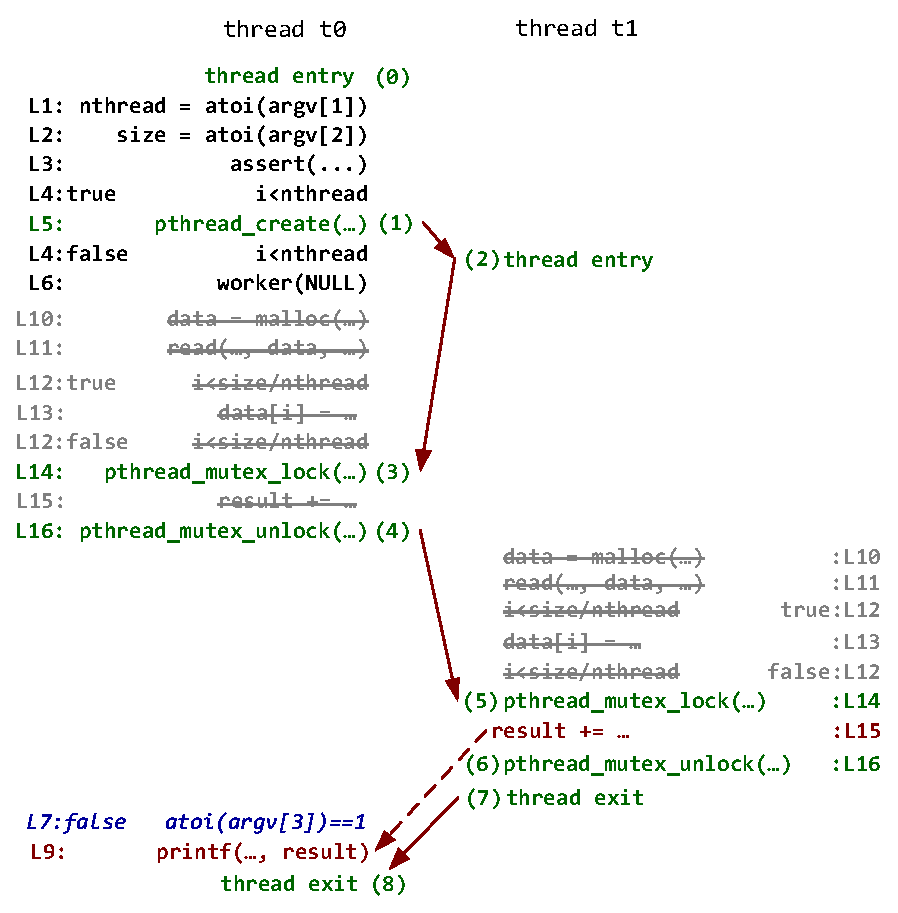
\includegraphics[width=\textwidth]{peregrine/figures/trace}
\end{minipage}
\caption{{\em Execution trace, hybrid schedule, and trace slice.}  An
  execution trace of the program in Figure~\ref{fig:example} on arguments
  ``\v{2 2 0}'' is shown.  Each executed instruction is tagged
  with its static line number L$i$.  Branch instructions are also tagged
  with their outcome (true or false).  Synchronization operations (green),
  including thread entry and exit, are tagged
  with their relative positions in the synchronization order.  They form a
  sync-schedule whose order constraints are shown with solid arrows.  L15 of
  thread $t_1$ and L9 of thread $t_0$ race on \v{result}, and this race is
  deterministically resolved by enforcing an execution order constraint
  shown by the dotted arrow.  Together, these order constraints form a hybrid
  schedule.  Instruction L7 of $t_0$ (italic and blue) is included in the
  trace slice to avoid new races, while L6, L4:false, L4:true, L3, L2, and
  L1 of $t_0$ are included due to intra-thread
  dependencies. Crossed-out (gray) instructions are elided from the
  slice.}\label{fig:trace}
\end{figure}

%% \begin{figure}[t]
%% \centering
%% \begin{minipage}[t]{.5\textwidth}
%% \begin{small}
%% $\underline{B_{t_0}}\,1_{t_0}\,2_{t_0}\,3_{t_0}\,4_{t_0}^T\,
%%   \underline{5_{t_0}}\,\underline{B_{t_1}}\,4_{t_0}^F\,
%%   6_{t_0}\,10_{t_0}\,11_{t_0}\,12_{t_0}^T\,13_{t_0}\,12_{t_0}^F\,
%%   \underline{14_{t_0}}\,\\
%%   15_{t_0}\,\underline{16_{t_0}}\,10_{t_1}\,11_{t_1}\,12_{t_1}^T\,13_{t_1}\,
%%   12_{t_1}^F\,\underline{14_{t_1}}\,\mathbf{15_{t_1}}\,\underline{16_{t_1}}\,
%%   \underline{E_{t_1}}\,7_{t_0}^F\,\mathbf{9_{t_0}}\,\underline{E_{t_0}}$
%% \end{small}
%% \end{minipage}
%% \caption{{\em An execution trace of Figure~\ref{fig:example} on arguments
%%     ``\v{2 2 0}.''}  We use $l_{t_i}$ to represent a dynamic instance of
%%   the instruction at line $l$ in Figure~\ref{fig:example} run by thread
%%   $t_i$.  If the instruction is a branch instruction, we also indicate
%%   whether the true branch (\eg, $4_{t_0}^T$) or the false branch (\eg,
%%   $4_{t_0}^F$) is taken. $B_{t_i}$ is the begin of thread $t_i$, and
%%   $E_{t_i}$ the end.  All synchronization operations are underlined. The
%%   two accesses to \v{result} that race are in bold.} \label{fig:trace}
%% \end{figure}

%% \begin{figure}[h]
%% \centering
%% 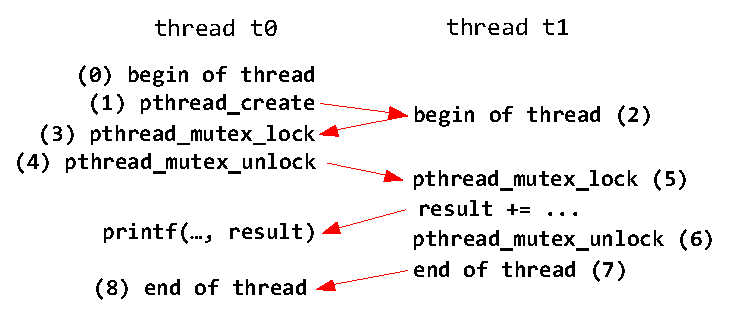
\includegraphics[width=.45\textwidth]{figures/example-schedule}
%% \caption{{\em Hybrid schedule extracted from Figure~\ref{fig:trace}.}
%%   Numbers in parenthesis are the indexes of the synchronization operations
%%   in the schedule; these indexes are used for detecting races
%%   (\S\ref{sec:schedule}). }\label{fig:example-schedule}
%% \end{figure}

%% \begin{figure}[t]
%% \centering
%% \begin{minipage}[t]{.5\textwidth}
%% \begin{small}
%% $thread\ t_0: \underline{B_{t_0}}\,1_{t_0}\,2_{t_0}\,3_{t_0}\,4_{t_0}^T\,
%%   \underline{5_{t_0}}\,4_{t_0}^F,6_{t_0}\,\underline{14_{t_0}}\,
%%   \underline{16_{t_0}}\,\hat{7_{t_0}^F}\,\mathbf{9_{t_0}}\,\underline{E_{t_0}}
%%   \\ thread\ t_1:
%%   \underline{B_{t_1}}\,\underline{14_{t_1}}\,\mathbf{15_{t_1}}\,\underline{16_{t_1}}\,
%%   \underline{E_{t_1}}$
%% \end{small}
%% \end{minipage}
%% \caption{{\em Trace slice computed from Figure~\ref{fig:trace}.} It
%%   consists of a path slice per thread.  Notation is identical to
%%   Figure~\ref{fig:trace} except the branch added for avoiding new races is
%%   with a hat ($\hat{7_{t_0}^F}$).} \label{fig:slice}
%% \end{figure}

\para{Recorder: execution trace.}
When we run the instrumented program with arguments ``\v{2 2 0}'' to spawn
two threads and process two bytes of data, suppose that the recorder records
the execution trace in Figure~\ref{fig:trace}.  (This figure also shows
the hybrid schedule and preconditions \peregrine computes, explained
later in this subsection.)  This trace is just one
possible trace depending on the scheduling algorithm the recorder uses.
% We will use the same notation defined in the figure caption to refer to
% dynamic instruction instances in the remainder of the paper.

%% We use $l_{t_i}$ to represent a dynamic instance of the instruction at
%% line $l$ in Figure~\ref{fig:example} run by thread $t_i$.  If the
%% instruction is a branch instruction, we also indicate whether the true
%% branch (\eg, $3_{t_0}^T$) or the false branch (\eg, $3_{t_0}^F$) is
%% taken. $B_{t_i}$ is the begin of thread $t_i$, and $E_{t_i}$ the end.
%% All synchronization operations are underlined.


% because the recorder can use different schedule algorithms and it does
% not enforce order
%% is configured to schedule synchronization operations using round-robin,
%% and it records an execution trace as shown in Figure~\ref{fig:trace}.
%% A round-robin algorithm ensures that the synchronization operations in
%% this example ($5_0,10_1,14_0,16_0,14_1$, and $16_1$) occur always in
%% this order.  ($10_1$ is the entry to thread 1; we explain why \peregrine
%% considers thread entry a synchronization event in
%% \S\ref{sec:instrument}.)  Since our recorder currently enforces no
%% order constraints for non-synchronization instructions, the above trace
%% is just one of the possible traces.

%$B_{t_0}5_{t_0}B_{t_1}14_{t_0}16_{t_0}14_{t_1}16_{t_1}E_{t_1}E_{t_0}$
\para{Analyzer: hybrid schedule.}
Given the execution trace, the analyzer starts by computing a hybrid
schedule.  It first extracts a sync-schedule consisting of the operations
tagged with (1), (2), ..., (8) in Figure~\ref{fig:trace}.  It then detects races in
the trace according to this sync-schedule, and finds the race on
\v{result} between L15 of thread $t_1$ and L9 of $t_0$.  It then computes an
execution order constraint to deterministically resolve this race, shown
as the dotted arrow in Figure~\ref{fig:trace}.  The sync-schedule and
execution order constraint together form the hybrid schedule.  Although
this hybrid schedule constrains the order of synchronization and the last
two accesses to \v{result}, it can still be efficiently reused because the
core computation done by \v{worker} can still run in parallel.

%% \begin{figure}[t]
%% \lgrindfile{code/simple.cpp.tex}
%% \caption{{\em Simplifications done by the analyzer to Figure~\ref{fig:example}.}} \label{fig:simple}
%% \end{figure}

\para{Analyzer: simplified program.}
To improve analysis precision, the analyzer simplifies the program according to the
hybrid schedule.  For instance, based on the number of
\v{pthread\_create()} operations in the schedule, the analyzer
% since this schedule has only one \v{pthread\_create()} call, the analyzer infers that \v{nthread} must be \v{2}, and unrolls the loop at line 4--5.  It also 
clones function \v{worker()} to give each thread a copy,
so that the alias analysis separates different threads and determines that
the two instances of L13 in $t_0$ and $t_1$ access different
\v{malloc}'ed locations and never race.

%% With cloning, the analyzer can infer that the two instances of \v{upriv}
%% are not alias.  In addition, it can compute the bounds for the loop at
%% line 22--26 for each thread function clone, and infer that the accesses to
%% \v{data} from different threads do not alias.

% It also clones \v{SlaveStart()} for each thread so that alias analysis
% does not merge results from different threads together.  These
% simplifications enable further simplifications, such as constant folding
% of the \v{SlaveStart\_clone*} arguments.  Figure~\ref{fig:simple} shows
% the simplification results.

\para{Analyzer: trace slice.}
The analyzer uses
determinism-preserving slicing to reduce the execution trace into a trace
slice, so that it can compute relaxed preconditions.
The final trace slice consists of the instructions not crossed out
in Figure~\ref{fig:trace}.
% shows the resultant trace slice with one \emph{path   slice} for each thread.
The analyzer computes this trace slice using inter-thread and 
intra-thread steps.  In the inter-thread step, it adds instructions
required to avoid new races into the slice.  Specifically, for $t_0$ it adds
the false branch of L7, or L7:false, because if the true branch
is taken, a new race between L8 of $t_0$ and L15 of $t_1$ occurs.  It
ignores branches of line L12 because alias analysis already determines that L13 of
$t_0$ and L13 of $t_1$ never race.

In the intra-thread step, the analyzer adds instructions required 
to reach all instructions identified in the
inter-thread step (L7:false of $t_0$ in this example) and all events in
the hybrid schedule.  It does so by traversing the execution trace
backwards and tracking control- and data-dependencies.  In this example, it
removes L15, L13, L12, L11, and L10 because no instructions currently in
the trace slice depend on them.  It adds L6 because without this call, the
execution will not reach instructions L14 and L16 of thread $t_0$.  It adds
L4:false because if the true branch is taken, the execution of $t_0$ will
reach one more \v{pthread\_create()}, instead of L14,
\v{pthread\_mutex\_lock()}, of $t_0$.  It adds L4:true because this branch
is required to reach L5, the \v{pthread\_create()} call.  It similarly
adds L3, L2, and L1 because later instructions in the trace slice
depend on them.

%% It filters $2_{t_0}$ because no instruction in $t_0$'s path slice
%% depends on $2_{t_0}$.  Finally, it adds $1_{t_0}$ because $3_{t_0}^{T/F}$
%% uses variable \v{nthread} defined by $1_{t_0}$.

%% is in the schedule and depends on $3_{t_0}$.  

% thread exit actually can be ignored as long as we always call
% pthread_join during both recording and replay if the program calls
% pthread_join

\para{Analyzer: preconditions.}
After slicing, all branches from L12 are gone.  The
analyzer joins the remaining branches together as the
preconditions, using a version of \klee~\cite{klee:osdi08} augmented with
thread support~\cite{cui:tern:osdi10}.  Specifically, the analyzer marks
input data as \emph{symbolic}, and then uses \klee to track how this symbolic
data is propagated and observed by the instructions in the trace slice.
(Our \peregrine prototype runs symbolic execution within the recorder for
simplicity; see \S\ref{sec:record}.)
If a branch instruction inspects symbolic data and proceeds down the true
branch, the analyzer adds the precondition that the symbolic data makes
the branch condition true.  The analyzer uses symbolic
summaries~\cite{castro:bouncer} to succinctly generalize common library
functions.  For instance, it considers the return of \v{atoi(arg)}
symbolic if \v{arg} is symbolic.

\begin{figure}[t]
\centering
\begin{minipage}[t]{3.1in}
\begin{scriptsize}
$(atoi\_argv_1 = 2) \wedge (atoi\_argv_2 \geq atoi\_argv_1) \wedge
  (atoi\_argv_3 \neq 1) $
\end{scriptsize}
\end{minipage}
\caption{{\em Preconditions computed from the trace slice in
    Figure~\ref{fig:trace}.}  Variable $atoi\_argv_i$ represents the
  return of \v{atoi(arg[i])}.} \label{fig:precond}
\end{figure}

Figure~\ref{fig:precond} shows the preconditions the analyzer computes
from the trace slice in Figure~\ref{fig:trace}.
These preconditions illustrate two key benefits of \peregrine.
First, they are sufficient to ensure deterministic reuses of the schedule.
Second, they only loosely constrain the data size ($atoi\_argv_2$) and do
not constrain the data contents (from \v{read()}), allowing frequent
schedule-reuses.  The reason is that L10--L13 are all sliced out.
One way to leverage this benefit is to populate a
schedule cache with small workloads to reduce analysis time, and then
reuse the schedules on large workloads.

%% Third, these preconditions are still not the \emph{weakest
%%   preconditions}~\cite{aho:dragon:06} (\ie, most relaxed preconditions).
%% For instance, they require that \v{argv[3]} has a valid length of one
%% (excluding the terminating non-digit characters).  In general, computing
%% weakest preconditions is undecidable~\cite{aho:dragon:06}, so we
%% explicitly designed \peregrine to compute sufficient preconditions which may
%% still include unnecessary ones.

%% The preconditions on $argv_{i,1}$ (byte 1 of \v{argv[i]}) are collected
%% from the body of \v{atoi()} as \klee comes with a \v{Libc} implementation.


% Although we may further relax these preconditions using a string
% solver~\cite{hampi:issta09},

\para{Replayer.}
%The analyzer finishes by storing the hybrid schedule in 
%Figure~\ref{fig:trace} and the preconditions
%in Figure~\ref{fig:precond} into a schedule cache.
Suppose we run this program again on different arguments ``\v{2 1000 8}.''
The replayer checks the new arguments against the preconditions in
Figure~\ref{fig:precond} using \klee's constraint checker, and finds that these
arguments satisfy the preconditions, despite the much larger data size.  
It can therefore reuse the hybrid schedule in Figure~\ref{fig:trace}
on this new input by enforcing
the same order of synchronization operations and accesses
% (L15 of $t_1$ and L9 of $t_0$)
to \v{result}.

%  Specifically, it schedules the synchronization wrappers based on the
%  schedule, and enforces the order constraints to resolve the races on
%  \v{result} using a fast instrumentation framework we previously built.

%% This example illustrates four benefits of \peregrine.  First, despite that \peregrine
%% enforces a hybrid schedule, the core computation done by \v{worker} can
%% still run in parallel.  

%% Second, the preconditions it computes ensures
%% deterministic reuse of schedules.


% and we explicitly design \peregrine to soundly compute sufficient
% preconditions.



%% \peregrine then computes the preconditions \v{argv[1][0]=='2' \&\&
%%   argv[1][1]==0}, and inserts the schedule and preconditions into the
%% schedule cache.  It can reuse this schedule whenever we run the code in
%% Figure~\ref{fig:example} with two threads (\v{argv[1]} is ``2'').


%% Figure~\ref{fig:analyzer} shows all analysis it performs to
%% compute these two key pieces of data.  To compute a hybrid schedule, the
%% analyzer first extracts a total order of synchronization operations from
%% the execution trace into the schedule.  It then detects data races with
%% respect to this extracted synchronization order, and adds additional
%% execution order constraints to the schedule to deterministically resolve
%% the detected races (\S\ref{sec:schedule}).

%% To compute the preconditions of a schedule, the analyzer first
%% \emph{simplifies} the program according to the schedule.  For instance, it
%% clones functions to give each thread in the schedule its own copies of the
%% functions.  It does so because alias analysis often cannot distinguish
%% dynamic instances of threads, and often imprecisely merge results from
%% multiple threads into one.  This cloning significantly improves precision
%% because a common idiom in multithreaded programs is to share the same
%% functions among a set of worker threads.

%% The analyzer then computes alias results from the simplified program.
%% Given the alias results and the schedule computed above, the analyzer
%% \emph{slices} the execution trace into a \emph{trace slice} with much
%% fewer conditionals while preserving determinism.  The analyzer does so in
%% an inter- and an intra-thread steps.  In the inter-thread step, it starts
%% by computing \emph{input-dependent} races that does not occur in the
%% execution trace, but may occur if we reuse the schedule on a different
%% input.  It then avoids these input-dependent races by including certain
%% branches in the trace slice or adding additional preconditions.  For
%% instance, to avoid the input-dependent race in
%% Figure~\ref{fig:input-race}, \peregrine would require that the false branch of
%% the \v{if}-statement is always taken, which effectively adds a
%% precondition $x \neq 0$.  In the intra-thread step, the analyzer runs a
%% slightly modified precondition slicing algorithm to compute a path slice
%% within each thread to ensure that all events in the schedule and all
%% targets identified in the inter-thread step are reachable.

%% Given a trace slice with much fewer conditionals than the execution trace,
%% the analyzer runs \emph{symbolic
%%   execution}~\cite{klee:osdi08,castro:bouncer,cui:tern:osdi10} to
%% conceptually conjunct the input-dependent conditionals together as the
%% preconditions.  The specific symbolic execution engine we use is
%% \klee~\cite{klee:osdi08}.  

%% Once the analyzer finishes, it computes a $\langle C, S \rangle$ tuple where $S$
%% is a schedule and $C$ is the preconditions of the schedule.  All $\langle
%% C, S \rangle$ are stored into a schedule cache, which the \emph{replayer}
%% uses to run a program.  Specifically, when an input arrives, the replayer
%% searches the schedule cache for a $\langle C, S \rangle$ tuple such that
%% the input satisfies the preconditions $C$.  If it finds such a tuple, it
%% simply runs the program enforcing schedule $S$.  Otherwise, it switches to
%% the recorder, which records an execution trace so that the analyzer can
%% relax the trace into a schedule.  To speed up this search, \peregrine organizes
%% the schedule cache as a tree, instead of a flat
%% set~\cite{cui:tern:osdi10}.

%% For clarity, we will present the core program analysis techniques
%% (\S\ref{sec:slice} and \S\ref{sec:guide}) at the source level.

\subsection{Deployment and Usage Scenarios} \label{sec:deploy}

\peregrine runs in user-space and requires no special hardware, presenting few
challenges for deployment.  To populate a schedule cache, a user can
record execution traces from real workloads;
% , and run \peregrine to compute schedules;
or a developer can run (small) representative workloads
to pre-compute schedules before deployment.  \peregrine
efficiently makes the behaviors of multithreaded programs more repeatable,
even across a range of inputs.  We envision that users can use this repeatability in
at least four ways.

\para{Concurrency error avoidance.} \peregrine can reuse well-tested schedules
collected from the testing lab or the field, reducing the risk of running
into untested, buggy schedules.  
Currently \peregrine detects and avoids only data races.  However, combined with
the right error detectors, \peregrine can be easily extended to detect and
avoid other types of concurrency errors.

\para{Record and replay.} Existing deterministic record-replay systems
tend to incur high CPU and storage overhead (\eg, 15X
slowdown~\cite{idna:vee06} and 11.7 GB/day
storage~\cite{smp-revirt:vee08}).  A record-replay system on top of \peregrine
may drastically reduce this overhead: for inputs that hit the
schedule cache, we do not have to
log any schedule.
%efficiently reuse a deterministic schedule without logging synchronization operations or memory accesses.
% For inputs that miss, the overhead with \peregrine should be comparable to as
% existing tools, but we assume cache-hits to dominate (\S\ref{sec:}).

\para{Replication.}  % A replication tool tolerates faults by running
% multiple replicas of a program.  However,
To keep replicas of a multithreaded program consistent, a replication tool
often records the thread schedules at one replica and replays them at
others.  This technique is essentially \emph{online}
replay~\cite{respec:asplos10}.
% as opposed to offline replay described above.  
It may thus incur high CPU, storage, and
bandwidth overhead.  With \peregrine, replicas can maintain a consistent
schedule cache.  If an input hits the schedule cache, all replicas will
automatically select the same deterministic schedule, incurring zero
bandwidth overhead.

\para{Schedule-diversification.}  Replication can tolerate
hardware or network failures, but the replicas may still run into the same
concurrency error because they all use the same schedules.  Fortunately,
many programs are already ``mostly-deterministic'' as they either compute
the same correct result or encounter heisenbugs.  We can thus run \peregrine to
deterministically diversify the schedules at different replicas (\eg,
using different scheduling algorithms or schedule caches) to tolerate
\emph{unknown} concurrency errors,

\para{Applications of individual techniques.} The individual ideas in \peregrine
can also benefit other research efforts.  For instance, hybrid schedules
can make the sync-schedule approach deterministic without recording
executions, by coupling it with a sound static race detector.
Determinism-preserving slicing can (1) compute input filters to block bad
inputs~\cite{castro:bouncer} causing concurrency errors and (2) randomize
an input causing a concurrency error for use with anonymous bug
reporting~\cite{castro:bug-report-privacy}.  Schedule-guided
simplification can transparently improve the precision of many existing
static analyses: simply run them on the simplified programs.  This improved
precision may be leveraged to accurately detect errors or even
verify the correctness of a program according to a set of schedules.
Indeed, from a verification perspective, our simplification technique
helps \emph{verify} that executions reusing schedules have \emph{no}
new races.

